\documentclass{beamer}

\usepackage{comment}
\usepackage{color}
\usepackage{listings}
\usepackage{verbatim}
\usepackage{multicol}
\usepackage{booktabs}
\definecolor{green}{RGB}{0,128,0}

\newcommand\gehcomment[1]{{{\color{orange} #1}}}
\newcommand\add[1]{{{\color{blue} #1}}}
\newcommand\remove[1]{\sout{{\color{red} #1}}}
\newcommand\codecomment[1]{{{\color{green} #1}}}
\newcommand\redcomment[1]{{{\color{red} #1}}}
\newcommand\bluecomment[1]{{{\color{blue} #1}}}
\newcommand\greencomment[1]{{{\color{green} #1}}}
\newcommand\magentacomment[1]{{{\color{magenta} #1}}}

\begin{comment}
\tiny
\scriptsize
\footnotesize
\small
\normalsize
\large
\Large
\LARGE
\huge
\Huge
\end{comment}

\begin{document}
\title{Multiphase - Gas Injection}
\author{Emily Stein}
\date{\today}

%\frame{\titlepage}

%-----------------------------------------------------------------------------
\section{Location of Example}

\begin{frame}[fragile,containsverbatim]\frametitle{Location}

Location of this example problem:

\begin{semiverbatim}
> cd \$PFLOTRAN_DIR
> cd shortcourse/exercises/gas_injection
> ls

gas_injection.in
gas_injection.py
\end{semiverbatim}

\end{frame}

%-----------------------------------------------------------------------------
\subsection{Command Line}
\begin{frame}[fragile]\frametitle{Command Line}
This problem takes a few minutes, so let's begin the simulation now.

\begin{itemize}
  \item Run the simulation
\end{itemize}

\begin{semiverbatim}
> cd \$PFLOTRAN_DIR
> cd shortcourse/exercises/gas_injection
> pflotran -input_prefix gas_injection
\end{semiverbatim}

\end{frame}

%-----------------------------------------------------------------------------
\section{Description of Gas Injection}

\subsection{Gas Injection Conceptual Model}

\begin{frame}\frametitle{Description of Gas Injection Scenario}
The ``Gas Injection Scenario'' demonstrates how to set up a multiphase flow simulation using \redcomment{GENERAL MODE}. It simulates gas injection into a 2D liquid-saturated domain. Assumptions include:
\begin{itemize}
  \item Problem domain: $100 \times 1 \times 100$ m (x $\times$ y $\times$ z)
  \item Grid resolution: $5 \times 1 \times 5$ m 
  \item Flow mode: General
  \item Gas Source: Rate scaled by cell volume
  \item Maximum time step size: changes with simulation time
  \item Total simulation time: 100 y
\end{itemize}

\end{frame}

%-----------------------------------------------------------------------------
\frame{\frametitle{2D Gas Injection Scenario Schematic}
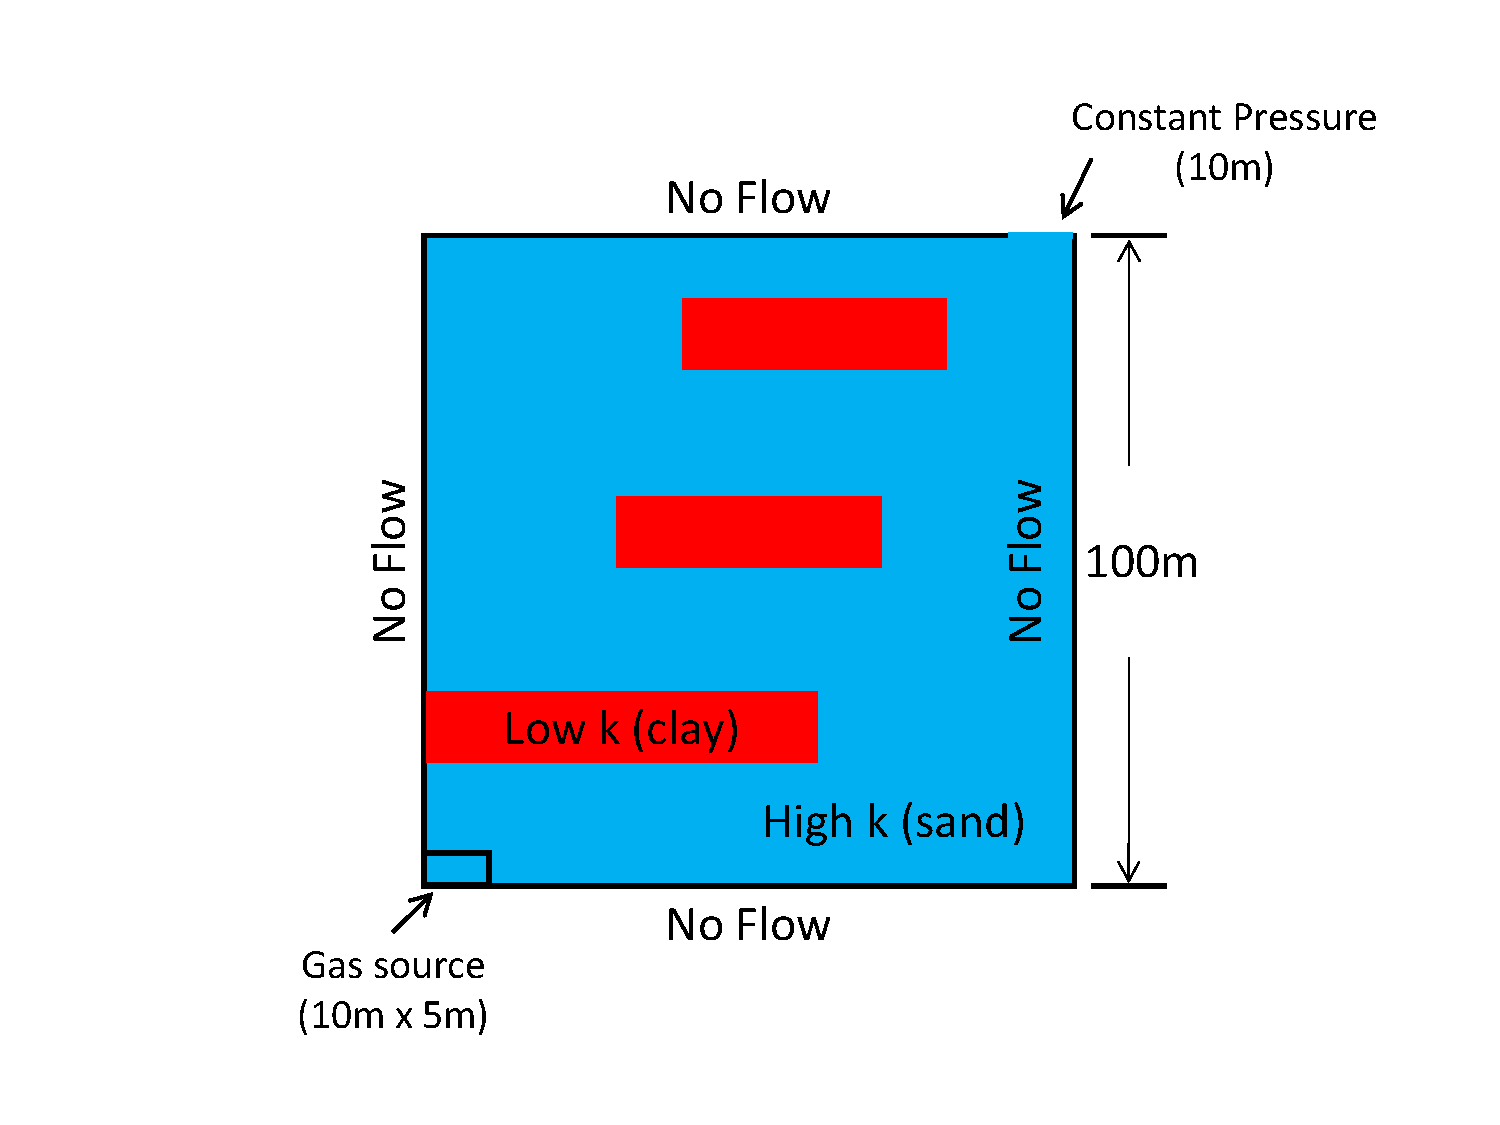
\includegraphics[width=\linewidth]{./gas_injection_bc}
}

%-----------------------------------------------------------------------------
\frame{\frametitle{2D Gas Injection Initial Conditions}
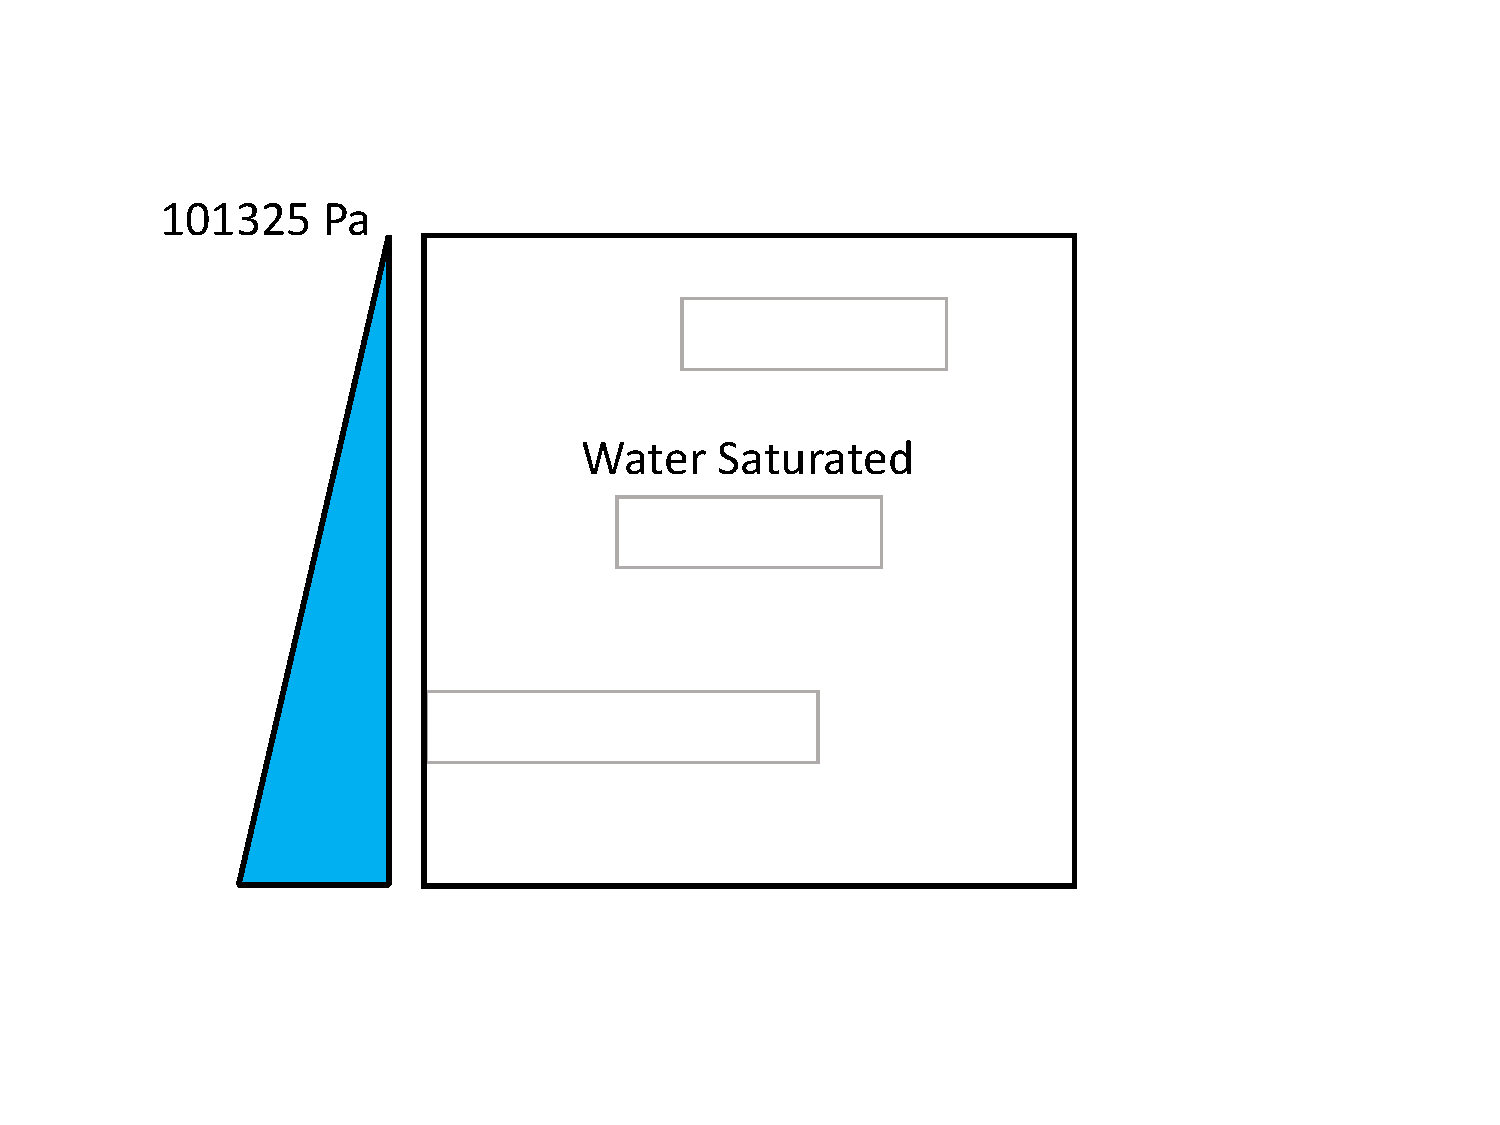
\includegraphics[width=\linewidth]{./gas_injection_ic}
}

%-----------------------------------------------------------------------------
\section{Description of Input Deck}

%-----------------------------------------------------------------------------
\subsection{SIMULATION}

\begin{frame}[fragile]\frametitle{SIMULATION}

\begin{itemize}
  \item Multiphase flow (\redcomment{General mode})
  \item with \redcomment{options}
\end{itemize}

\begin{semiverbatim}\small
SIMULATION
  SIMULATION_TYPE SUBSURFACE
  PROCESS_MODELS
    SUBSURFACE_FLOW flow
      MODE GENERAL \bluecomment{! two-phase flow and energy}
      OPTIONS
        GAS_COMPONENT_FORMULA_WEIGHT 44.d0 \bluecomment{! CO2(g)} 
        ISOTHERMAL \bluecomment{! ignore energy component}
      /   
    /   
  /
END

SUBSURFACE
...
END_SUBSURFACE
\end{semiverbatim}

\end{frame}

%-----------------------------------------------------------------------------
\subsection{GRID}

\begin{frame}[fragile]\frametitle{GRID}

\begin{itemize}
  \item Problem domain: $100 \times 1 \times 100$ m (x $\times$ y $\times$ z)
  \item Grid resolution: $5 \times 1 \times 5$ m
\end{itemize}

\begin{semiverbatim}
GRID
  TYPE STRUCTURED
  NXYZ 20 1 20         \bluecomment{! number of cells in x y z}
  BOUNDS
    0.d0 0.d0 0.d0     \bluecomment{! xmin ymin zmin}
    100.d0 1.d0 100.d0 \bluecomment{! xmax ymax zmax}
  /
END
\end{semiverbatim}

\end{frame}

%-----------------------------------------------------------------------------
\subsection{FLUID\_PROPERTY}

\begin{frame}[fragile]\frametitle{FLUID\_PROPERTY}
\begin{itemize}
  \item Diffusion of dissolved gas in \redcomment{liquid phase}
  \item Diffusion of water vapor in \redcomment{gas phase}
\end{itemize}

\begin{semiverbatim}

FLUID_PROPERTY
  PHASE LIQUID \bluecomment{! for diffusion of dissolved gas}
  DIFFUSION_COEFFICIENT 1.d-9
END

FLUID_PROPERTY
  PHASE GAS \bluecomment{! for diffusion of water vapor}
  DIFFUSION_COEFFICIENT 2.1d-5
END
\end{semiverbatim}

\end{frame}

%-----------------------------------------------------------------------------
\subsection{OUTPUT}

\begin{frame}[fragile]\frametitle{OUTPUT}
\begin{itemize}
  \item Print a \redcomment{snapshot} of entire solution periodically
  \item Print the solution at \redcomment{observation points} every time step
  \item Print \redcomment{mass balance} file every time step
  \item Choose output \redcomment{variables}
\end{itemize}

\end{frame}

\begin{frame}[fragile]\frametitle{OUTPUT}

\begin{semiverbatim}\small
OUTPUT
  SNAPSHOT_FILE
    FORMAT HDF5
    PERIODIC TIME 0.01 y between 0. y and .1 y \bluecomment{! every 0.01 y}
    PERIODIC TIME 0.1 y between 0. y and 5. y  \bluecomment{! then 0.1 y}
    PERIODIC TIME 1. y between 0. y and 30. y  \bluecomment{! etc.}
    PERIODIC TIME 10. y between 0. y and 100. y
  /
  OBSERVATION_FILE
    PERIODIC TIMESTEP 1 \bluecomment{! print every time step}
  /
  MASS_BALANCE_FILE
    PERIODIC TIMESTEP 1 \bluecomment{! print every time step}
  /
  VELOCITY_AT_CENTER \bluecomment{! of cell}
  VARIABLES
    LIQUID_SATURATION
    GAS_SATURATION \bluecomment{! see input deck for more}
  /
END
\end{semiverbatim}

\end{frame}

%-----------------------------------------------------------------------------
\subsection{TIME}

\begin{frame}[fragile]\frametitle{TIME}
\begin{itemize}
  \item \redcomment{Final} simulation \redcomment{time} = 100 y
  \item \redcomment{Maximum time step size} = 5 y
\end{itemize}

\begin{semiverbatim}

TIME
  FINAL_TIME 100.d0 y \bluecomment{! end of simulation}
  MAXIMUM_TIMESTEP_SIZE 0.05 y at 0. y \bluecomment{! start small}
  MAXIMUM_TIMESTEP_SIZE 0.5 y at 5. y \bluecomment{! allow larger}
  MAXIMUM_TIMESTEP_SIZE 5. y at 30. y \bluecomment{! at late times}
END
\end{semiverbatim}

\end{frame}

%-----------------------------------------------------------------------------
\subsection{MATERIAL\_PROPERTY}

\begin{frame}[fragile]\frametitle{MATERIAL\_PROPERTY}
\begin{itemize}
  \item Energy equations require:
  \begin{itemize}
    \item \redcomment{mineral density}
    \item \redcomment{thermal conductivity} (bulk wet and dry)
    \item \redcomment{mineral heat capacity}
  \end{itemize}
\end{itemize}

\begin{semiverbatim}
MATERIAL_PROPERTY sand \bluecomment{! define material} \greencomment{sand}
  ID 1
  CHARACTERISTIC_CURVES default
  POROSITY 0.20
  TORTUOSITY 0.58
  ROCK_DENSITY 2700. \bluecomment{! density of the solid phase}
  THERMAL_CONDUCTIVITY_DRY 1.0d0 \bluecomment{! dry bulk medium}
  THERMAL_CONDUCTIVITY_WET 3.1d0 \bluecomment{! wet bulk medium}
  HEAT_CAPACITY 830. \bluecomment{! heat capacity of the solid phase}
  PERMEABILITY
    PERM_ISO 1.d-13
  /
END
\end{semiverbatim}

\end{frame}

\begin{frame}[fragile]\frametitle{MATERIAL\_PROPERTY}

\begin{semiverbatim}
MATERIAL_PROPERTY clay \bluecomment{! define material} \greencomment{clay}
  ID 2
  CHARACTERISTIC_CURVES clay
  POROSITY 0.35
  TORTUOSITY 0.23
  ROCK_DENSITY 2700. \bluecomment{! kg/m3}
  THERMAL_CONDUCTIVITY_DRY 0.7d0 \bluecomment{! W/(m-K)}
  THERMAL_CONDUCTIVITY_WET 1.4d0 \bluecomment{! W/(m-K)}
  HEAT_CAPACITY 830. \bluecomment{! J/(kg-K)}
  PERMEABILITY
    PERM_ISO 1.d-19
  /
END
\end{semiverbatim}

\end{frame}
%-----------------------------------------------------------------------------
\subsection{CHARACTERISTIC\_CURVES}

\begin{frame}[fragile,containsverbatim]\frametitle{CHARACTERISTIC\_CURVES}

\begin{itemize}\small
  \item Van Genuchten \redcomment{saturation function}
  \item Mualem \redcomment{relative permeability} for liquid and gas phases
\end{itemize}

\begin{semiverbatim}\small
CHARACTERISTIC_CURVES default \bluecomment{! used with} \greencomment{sand}
  SATURATION_FUNCTION VAN_GENUCHTEN
    ALPHA 1.d-4
    M 0.5
    LIQUID_RESIDUAL_SATURATION 0.1d0
  /
  PERMEABILITY_FUNCTION MUALEM_VG_LIQ
    PHASE LIQUID
    M 0.5
    LIQUID_RESIDUAL_SATURATION 0.1d0
  /
  PERMEABILITY_FUNCTION MUALEM_VG_GAS
    PHASE GAS
    M 0.5
    LIQUID_RESIDUAL_SATURATION 0.1d0
    GAS_RESIDUAL_SATURATION 0.1d0
  /
END
\end{semiverbatim}

\end{frame}

\begin{frame}[fragile,containsverbatim]\frametitle{CHARACTERISTIC\_CURVES}

\begin{itemize}\small
  \item Van Genuchten \redcomment{saturation function}
  \item Mualem \redcomment{relative permeability} for liquid and gas phases
\end{itemize}

\begin{semiverbatim}\small
CHARACTERISTIC_CURVES clay \bluecomment{! used with} \greencomment{clay}
  SATURATION_FUNCTION VAN_GENUCHTEN
    ALPHA 7.d-7
    M 0.375
    LIQUID_RESIDUAL_SATURATION 0.1d0
  /
  PERMEABILITY_FUNCTION MUALEM_VG_LIQ
    PHASE LIQUID
    M 0.375
    LIQUID_RESIDUAL_SATURATION 0.1d0
  /
  PERMEABILITY_FUNCTION MUALEM_VG_GAS
    PHASE GAS
    M 0.375
    LIQUID_RESIDUAL_SATURATION 0.1d0
    GAS_RESIDUAL_SATURATION 0.1d0
  /
END
\end{semiverbatim}

\end{frame}
%-----------------------------------------------------------------------------
\subsection{REGION}

\begin{frame}[fragile]\frametitle{REGION}
Regions will be used for:
\begin{itemize}
  \item{assignment of \redcomment{BC} and \redcomment{IC}}
  \item{location of \redcomment{gas injection}}
  \item{assignment of \redcomment{material properties}}
\end{itemize}

\begin{semiverbatim}\small
REGION all               \bluecomment{! define region:} \greencomment{all}
  COORDINATES
    -1.d20 -1.d20 -1.d20 \bluecomment{! very large volume}
     1.d20  1.d20  1.d20 \bluecomment{! nothing will be left out}
  /
END

REGION upper_right       \bluecomment{! define region:} \greencomment{upper_right}
  FACE top               \bluecomment{! face for use in BC}
  COORDINATES
    90.d0 0.d0 100.d0
    100.d0 1.d0 100.d0
  /
END
\end{semiverbatim}
\end{frame}

\begin{frame}[fragile]\frametitle{REGION}

\begin{semiverbatim}\small
REGION lower_left        \bluecomment{! define region:} \greencomment{lower_left}
  COORDINATES            \bluecomment{! for gas injection}
    0.d0 0.d0 0.d0
    10.d0 1.d0 5.d0
  /
END

REGION clay1             \bluecomment{! define region:} \greencomment{clay1}
  COORDINATES            \bluecomment{! one of three clay regions}
    00.d0 0.d0 20.d0
    60.d0 1.d0 30.d0
  /
END

...

\end{semiverbatim}
  
\end{frame}
%-----------------------------------------------------------------------------
\subsection{OBSERVATION}

\begin{frame}[fragile]\frametitle{OBSERVATION}
\begin{itemize}
  \item{Define three more regions for \redcomment{output}}
\end{itemize}

\begin{semiverbatim}\small
REGION lower \bluecomment{! define region:} \greencomment{lower}
  COORDINATE 52.5 0.5 17.5 \bluecomment{! note single coordinate}
/

REGION middle \bluecomment{! define region:} \greencomment{middle}
  COORDINATE 52.5 0.5 47.5
/

REGION upper \bluecomment{! define region:} \greencomment{upper}
  COORDINATE 52.5 0.5 77.5
/
\end{semiverbatim}
\end{frame}

\begin{frame}[fragile]\frametitle{OBSERVATION}
\begin{itemize}
  \item{Use them as \redcomment{observation points}}
\end{itemize}

\begin{semiverbatim}\small
OBSERVATION
  REGION lower \bluecomment{! use} \greencomment{lower} \bluecomment{as obs pt}
/

OBSERVATION
  REGION middle \bluecomment{! use} \greencomment{middle} \bluecomment{as obs pt}
/

OBSERVATION
  REGION upper \bluecomment{! use} \greencomment{upper} \bluecomment{as obs pt}
/
\end{semiverbatim}
\end{frame}

%-----------------------------------------------------------------------------
\subsection{FLOW\_CONDITION}

\begin{frame}[fragile]\frametitle{FLOW\_CONDITION}
\begin{itemize}
  \item{Single phase liquid, hydrostatic}
  \item{Use for \redcomment{IC} and \redcomment{BC}}
\end{itemize}

\begin{semiverbatim}
FLOW_CONDITION saturated \bluecomment{! define }\greencomment{saturated} 
  TYPE                   \bluecomment{! single phase liquid}
    LIQUID_PRESSURE HYDROSTATIC
    MOLE_FRACTION DIRICHLET
    TEMPERATURE DIRICHLET
  /
  DATUM 0.d0 0.d0 100.d0  \bluecomment{! top of domain}
  LIQUID_PRESSURE 101325. \bluecomment{! Pa (atmospheric)}
  MOLE_FRACTION 1.d-8     \bluecomment{! dissolved gas}
  TEMPERATURE 25.d0       \bluecomment{! degrees C}
END
\end{semiverbatim}
\end{frame}

\begin{frame}[fragile]\frametitle{FLOW\_CONDITION}
\begin{itemize}
  \item{\redcomment{Source} term}
  \item{Use for gas injection}
\end{itemize}

\begin{semiverbatim}
FLOW_CONDITION gas_injection \bluecomment{! define }\greencomment{gas_injection} 
  TYPE
    RATE SCALED_MASS_RATE VOLUME \bluecomment{! volume averaged}
  /
       \bluecomment{! liquid gas energy}
  RATE 0.d0 1.d-4 0.d0 kg/s kg/s MW
END
\end{semiverbatim}
\end{frame}

%-----------------------------------------------------------------------------
\subsection{Couplers}

\begin{frame}[fragile]\frametitle{Couplers}

\begin{itemize}
  \item \redcomment{Initial condition}: flow condition \greencomment{saturated} with region \greencomment{all}
  \item \redcomment{Boundary condition}: flow condition \greencomment{saturated} with region \greencomment{upper\_right}
  \item \redcomment{Source}: flow condition \greencomment{gas\_injection} with region \greencomment{lower\_left}
\end{itemize}

\begin{semiverbatim}\small
\bluecomment{! initial condition}
INITIAL_CONDITION initial \bluecomment{! optional name}
  FLOW_CONDITION unsaturated
  REGION all
END
\bluecomment{! boundary condition}
BOUNDARY_CONDITION open \bluecomment{! optional name}
  FLOW_CONDITION saturated
  REGION upper_right
END
\bluecomment{! source or sink }
SOURCE_SINK gas \bluecomment{! optional name}
  FLOW_CONDITION gas_injection
  REGION lower_left
END
\end{semiverbatim}
\end{frame}

\begin{frame}[fragile]\frametitle{Couplers}

\begin{itemize}
  \item{Material \greencomment{sand} with region \greencomment{all}}
  \item{Material \greencomment{clay} with region \greencomment{clay1}}
  \item{etc. for regions \greencomment{clay2} and \greencomment{clay3}}
\end{itemize}

\begin{semiverbatim}\small
STRATA
  REGION all
  MATERIAL sand
END

STRATA         \bluecomment{! Overwrite previous}
  REGION clay1 \bluecomment{! one of three clay regions}
  MATERIAL clay
END

...
\end{semiverbatim}
\end{frame}

%-----------------------------------------------------------------------------
\subsection{END\_SUBSURFACE}
\begin{frame}[fragile]\frametitle{END\_SUBSURFACE}
\begin{itemize}
  \item Close the SUBSURFACE block
\end{itemize}

\begin{semiverbatim}
END_SUBSURFACE \bluecomment{That's all!}
\end{semiverbatim}
\end{frame}

%-----------------------------------------------------------------------------
\subsection{Command Line 2}
\begin{frame}[fragile]\frametitle{Command Line}

\begin{itemize}
  \item Plot the results
\end{itemize}

\begin{semiverbatim}
> python gas_injection.py
\end{semiverbatim}

\end{frame}

%-----------------------------------------------------------------------------
\subsection{Speed Up}
\begin{frame}[fragile]\frametitle{Can We Speed it Up?}

\begin{semiverbatim}
SIMULATION
  SIMULATION_TYPE SUBSURFACE
  PROCESS_MODELS
    SUBSURFACE_FLOW flow
      MODE GENERAL ! two-phase flow and energy
      OPTIONS
        RESTRICT_STATE_CHANGE
        GAS_COMPONENT_FORMULA_WEIGHT 44.d0 ! CO2
        ISOTHERMAL 
      /
    /
  /
END
\end{semiverbatim}

\begin{itemize}
  \item Plot the results
\end{itemize}

\begin{semiverbatim}
> python gas_injection.py
\end{semiverbatim}

\end{frame}

%-----------------------------------------------------------------------------
\subsection{Faster}
\begin{frame}[fragile]\frametitle{Faster?}

\begin{semiverbatim}
SIMULATION
  SIMULATION_TYPE SUBSURFACE
  PROCESS_MODELS
    SUBSURFACE_FLOW flow
      MODE GENERAL 
      OPTIONS
        RESTRICT_STATE_CHANGE
        ANALYTICAL_JACOBIAN
        GAS_COMPONENT_FORMULA_WEIGHT 44.d0 
        ISOTHERMAL 
      /
    /
  /
END
\end{semiverbatim}

\begin{itemize}
  \item Plot the results
\end{itemize}

\begin{semiverbatim}
> python gas_injection.py
\end{semiverbatim}

\end{frame}

%-----------------------------------------------------------------------------
\subsection{Faster2}
\begin{frame}[fragile]\frametitle{Faster!}

\begin{semiverbatim}
SIMULATION
  SIMULATION_TYPE SUBSURFACE
  PROCESS_MODELS
    SUBSURFACE_FLOW flow
      MODE GENERAL 
      OPTIONS
        RESTRICT_STATE_CHANGE
        ANALYTICAL_JACOBIAN
        USE_INFINITY_NORM_CONVERGENCE
        GAS_COMPONENT_FORMULA_WEIGHT 44.d0 
        ISOTHERMAL 
      /
    /
  /
END
\end{semiverbatim}

\begin{itemize}
  \item Plot the results
\end{itemize}

\end{frame}
%-----------------------------------------------------------------------------
\subsection{Faster3}
\begin{frame}[fragile]\frametitle{Faster!!}

\begin{semiverbatim}
SIMULATION
  SIMULATION_TYPE SUBSURFACE
  PROCESS_MODELS
    SUBSURFACE_FLOW flow
      MODE GENERAL 
      OPTIONS
        RESTRICT_STATE_CHANGE
        ANALYTICAL_JACOBIAN
        USE_INFINITY_NORM_CONVERGENCE
        REL_UPDATE_INF_TOL 1.d-2
        GAS_COMPONENT_FORMULA_WEIGHT 44.d0  
        ISOTHERMAL 
      /
    /
  /
END
\end{semiverbatim}

\begin{itemize}
  \item Plot the results
\end{itemize}

\end{frame}
%-----------------------------------------------------------------------------
\subsection{Faster4}
\begin{frame}[fragile]\frametitle{FASTER!!}

\begin{semiverbatim}
SIMULATION
  SIMULATION_TYPE SUBSURFACE
  PROCESS_MODELS
    SUBSURFACE_FLOW flow
      MODE GENERAL 
      OPTIONS
        RESTRICT_STATE_CHANGE
        ANALYTICAL_JACOBIAN
        USE_INFINITY_NORM_CONVERGENCE
        REL_UPDATE_INF_TOL 1.d0
        GAS_COMPONENT_FORMULA_WEIGHT 44.d0  
        ISOTHERMAL 
      /
    /
  /
END
\end{semiverbatim}

\end{frame}

%-----------------------------------------------------------------------------
\end{document}
